%%%%%%%%%%%%%%%%%%%%%%%%%%%%%%%%%%%%%%%%%%%%%%%%%%%%%%%%%%%%
%%  This Beamer template was created by Cameron Bracken.
%%  Anyone can freely use or modify it for any purpose
%%  without attribution.
%%
%%  Last Modified: January 9, 2009
%%

\documentclass[xcolor=x11names,compress]{beamer}

%% General document %%%%%%%%%%%%%%%%%%%%%%%%%%%%%%%%%%
\usepackage{graphicx}
\usepackage{tikz}
\usetikzlibrary{decorations.fractals}
%%%%%%%%%%%%%%%%%%%%%%%%%%%%%%%%%%%%%%%%%%%%%%%%%%%%%%

\usepackage{booktabs}


%% Beamer Layout %%%%%%%%%%%%%%%%%%%%%%%%%%%%%%%%%%
\useoutertheme[subsection=false,shadow]{miniframes}
\useinnertheme{default}
\usefonttheme{serif}
\usepackage{palatino}


\setbeamerfont{title like}{shape=\scshape}
\setbeamerfont{frametitle}{shape=\scshape}

\setbeamercolor*{lower separation line head}{bg=DeepSkyBlue4}
\setbeamercolor*{normal text}{fg=black,bg=white}
\setbeamercolor*{alerted text}{fg=red}
\setbeamercolor*{example text}{fg=black}
\setbeamercolor*{structure}{fg=black}

\setbeamercolor*{palette tertiary}{fg=black,bg=black!10}
\setbeamercolor*{palette quaternary}{fg=black,bg=black!10}

\renewcommand{\(}{\begin{columns}}
\renewcommand{\)}{\end{columns}}
\newcommand{\<}[1]{\begin{column}{#1}}
\renewcommand{\>}{\end{column}}
%%%%%%%%%%%%%%%%%%%%%%%%%%%%%%%%%%%%%%%%%%%%%%%%%%




\begin{document}


%%%%%%%%%%%%%%%%%%%%%%%%%%%%%%%%%%%%%%%%%%%%%%%%%%%%%%
%%%%%%%%%%%%%%%%%%%%%%%%%%%%%%%%%%%%%%%%%%%%%%%%%%%%%%
\section{\scshape Introduction}
\begin{frame}
\title{Reserve in Electricity Markets}
%\subtitle{SUBTITLE}
\author{
    Nigel Cleland\\
    {\it University of Auckland \\
    EPOC}\\
}
\date{

    \vspace{1cm}
    \today
}
\titlepage
\end{frame}

%%%%%%%%%%%%%%%%%%%%%%%%%%%%%%%%%%%%%%%%%%%%%%%%%%%%%%
%%%%%%%%%%%%%%%%%%%%%%%%%%%%%%%%%%%%%%%%%%%%%%%%%%%%%%
\begin{frame}{Introduction}
\tableofcontents
\end{frame}

\begin{frame}{About Me}
\begin{itemize}
\item University of Canterbury, BE(Hons) Chemical and Process Engineering
\item University of Auckland, Year Three, Ph.D Eng. Sci and C\&M
\item Prior work at load aggregators
\item HVDC Pole 3 Commissioning (Trading Team)
\item Based at Transpower S.O. 2013
\item Various Consulting Jobs
\end{itemize}
\end{frame}

\begin{frame}{Rough Agenda}
\begin{itemize}
\item Reserve Constraints
\item Assessment of Spot Prices
\item Equilibrium Models of Reserve Participants
\item Visualising Energy and Reserve Offers
\item Using Bayesian Probability to assess Constraints
\item Theoretical HVDC Transfer Capabilities
\item Open Source and Open Data
\end{itemize}
\end{frame}

%%%%%%%%%%%%%%%%%%%%%%%%%%%%%%%%%%%%%%%%%%%%%%%%%%%%%%
%%%%%%%%%%%%%%%%%%%%%%%%%%%%%%%%%%%%%%%%%%%%%%%%%%%%%%
\section{\scshape Reserve Constraints}
\begin{frame}{It starts with a picture}
\begin{figure}
%\includegraphics[width=0.95\textwidth]{}
\caption{Haywards Nodal Spot Price (x axis) compared with the North Island
FIR Price (y axis)}
\end{figure}
\end{frame}

%%%%%%%%%%%%%%%%%%%%%%%%%%%%%%%%%%%%%%%%%%%%%%%%%%%%%%
%%%%%%%%%%%%%%%%%%%%%%%%%%%%%%%%%%%%%%%%%%%%%%%%%%%%%%
\begin{frame}{Why does this matter?}
\begin{figure}
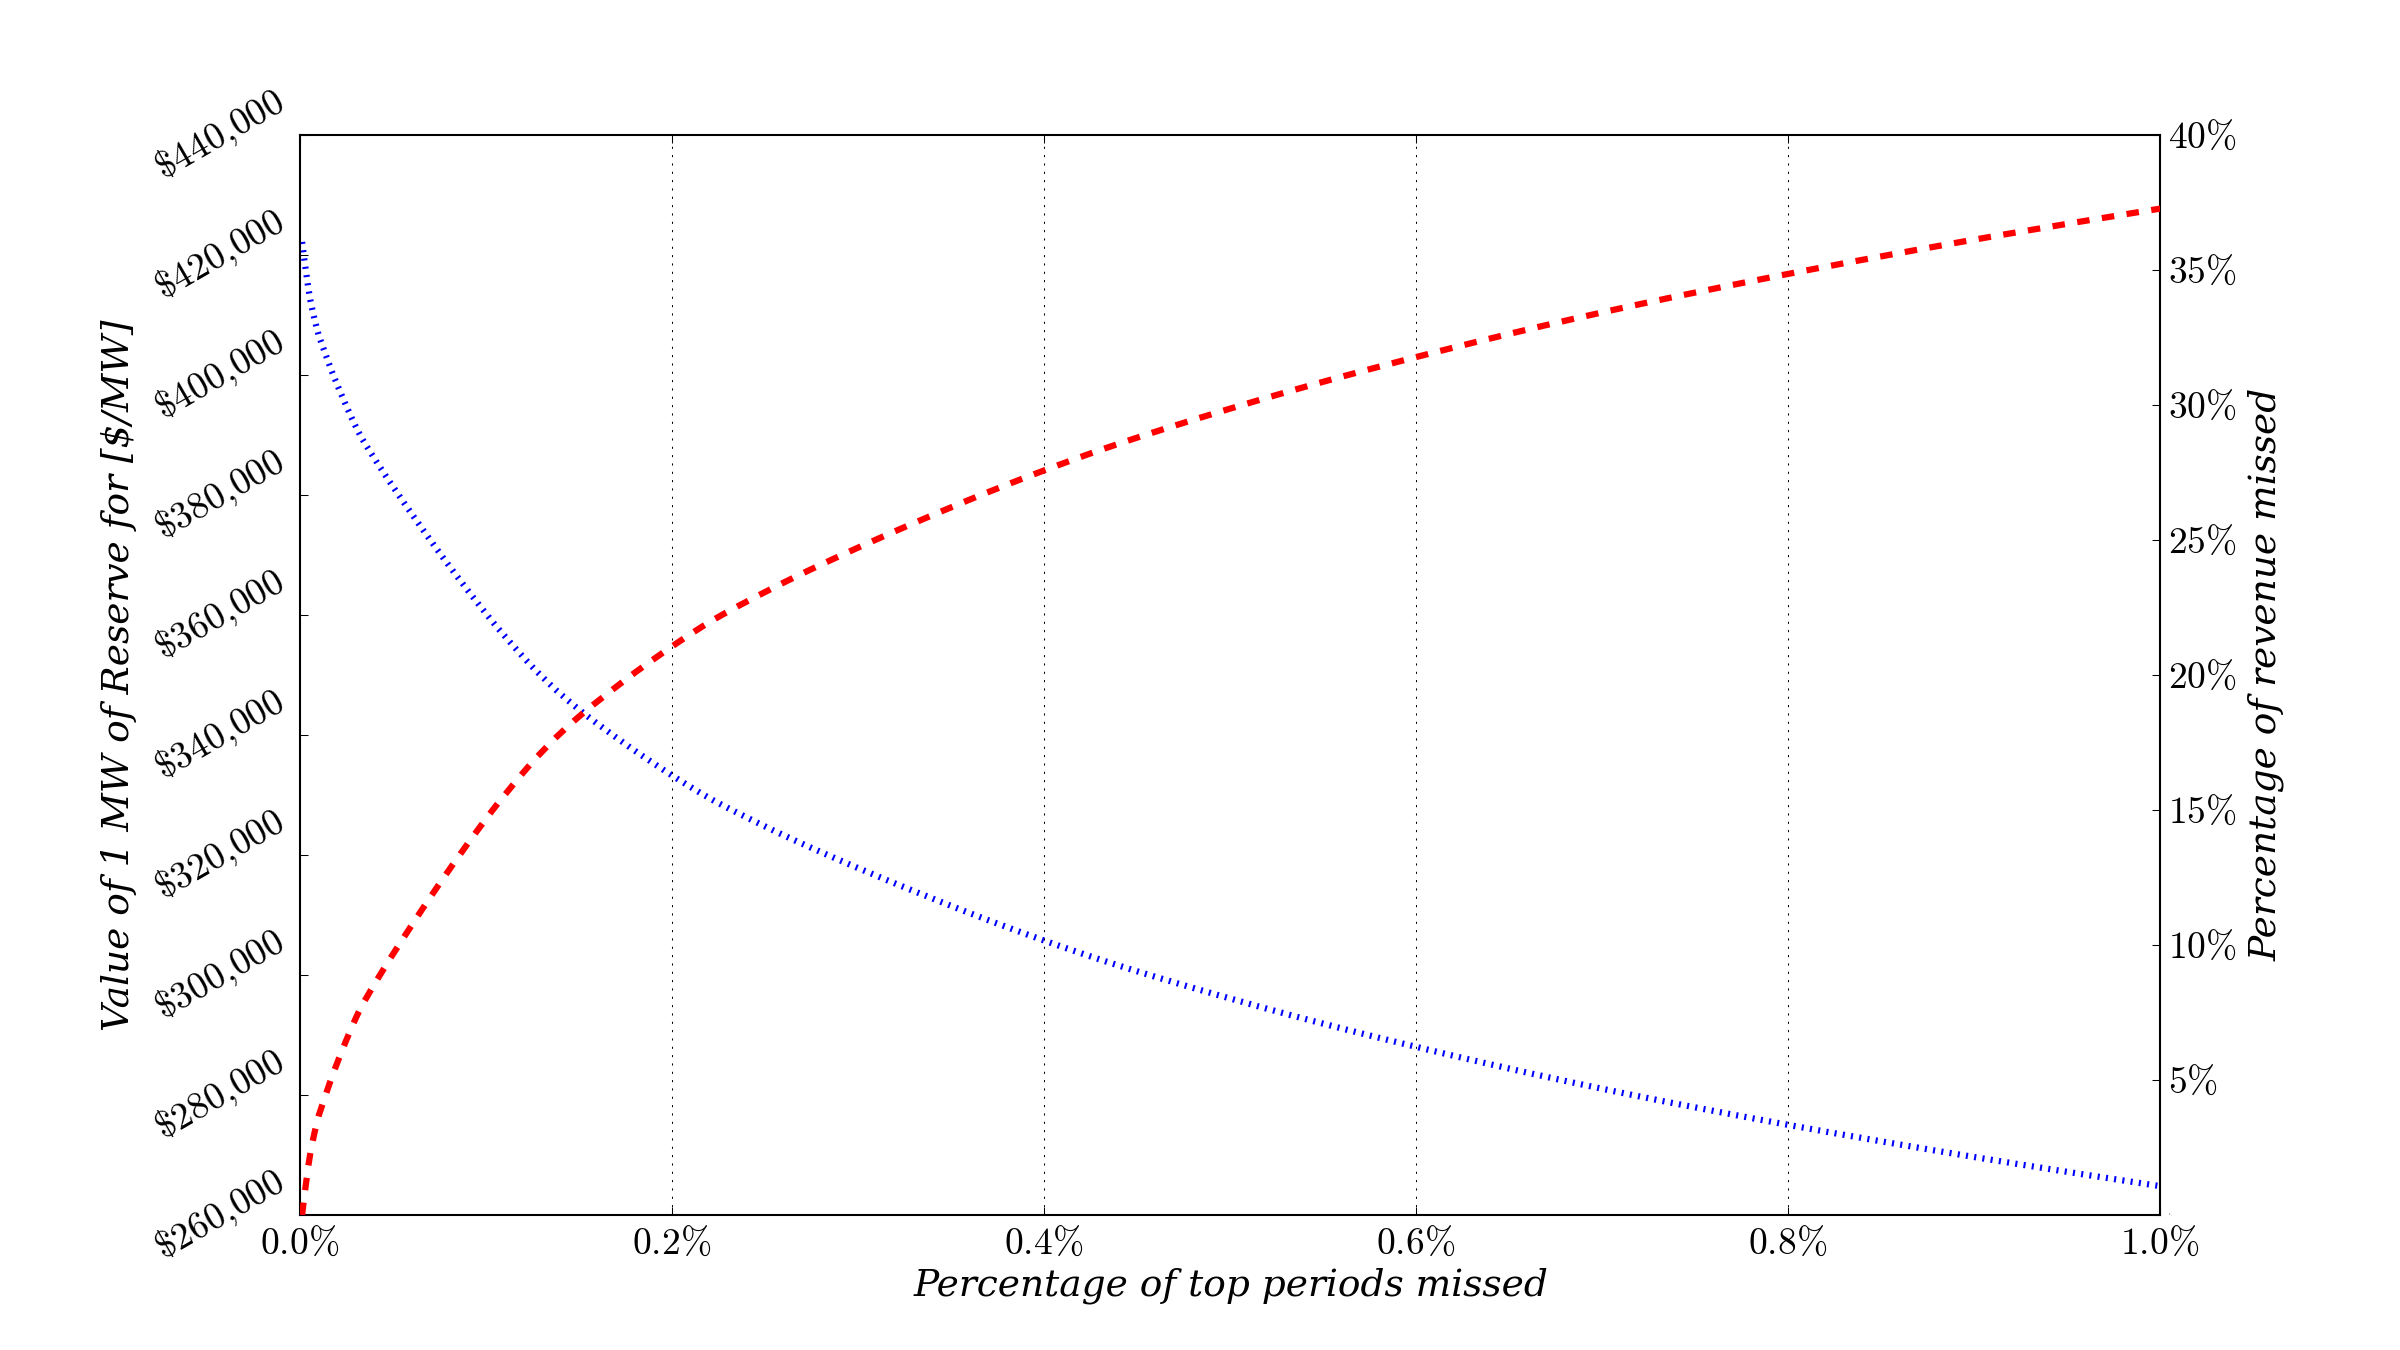
\includegraphics[width=0.95\textwidth]{img/reserveprice.png}
\caption{Revenue ``lost'' for missing highly priced trading periods}
\end{figure}
\end{frame}

\begin{frame}{Effect on Individual Consumers}
\begin{table}
\caption{Monthly Revenue ``missed'' by various IL producers}
\begin{tabular}{cccc}
\toprule
& NZST & PPAC & SKOG \\
\midrule
2009 & 18-85\% & 2-92\% & 30-80\% \\
2010 & 4-90\% & 0-90\% & 5-70\% \\
\bottomrule
\end{tabular}
\end{table}
In November 2010 NZST missed 90\% of the monthly IR Revenue, SKOG missed 6\%
\vspace{2cm}
\end{frame}

%%%%%%%%%%%%%%%%%%%%%%%%%%%%%%%%%%%%%%%%%%%%%%%%%%%%%%
%%%%%%%%%%%%%%%%%%%%%%%%%%%%%%%%%%%%%%%%%%%%%%%%%%%%%%
\begin{frame}{Some Theory}
\scalebox{0.75}{
\begin{minipage}{0.50\textwidth}
\begin{eqnarray*}
[POPF] \min & p_g^T g + p_r^T r & \\
\text{st.} &  Mg + Af = d &[\pi] \\
                  &  r + g \le G &[\epsilon] \\
                  &  r - Kg \le 0 &[\kappa]  \\
                  & Er - g \ge 0 &[\lambda^{1}] \\
                  & Hr - Bf \ge 0 &[\lambda^{2}] \\
                  & r \le R &[\omega] \\
                  & |f| \le F &[\tau^{\pm}] \\
                  & Lf  = 0 & [\alpha] \\
                  & r, g \geq 0 & \\
\end{eqnarray*}
\end{minipage}}
\scalebox{0.75}{
\begin{minipage}{0.3\textwidth}
\begin{eqnarray*}
[DOPF] \max & d^{T} + R^{T}\omega + G^{T}\epsilon + F^{T}(\tau^{+} +
\tau^{-}) & \\
\text{st.} & M^{T}\pi + \epsilon - K\kappa + \lambda^{1} \le p_g &[g] \\
                  & \omega + \epsilon + \kappa + E\lambda^{1} \le p_r &[r]  \\
                  & A^{T}\pi + \tau^{+} - \tau^{-} - B^{T}\lambda^{2} +L^{T}\alpha = 0  &[f] \\
                  & \omega, \epsilon, \tau^{\pm}, \kappa \le 0 & \\
                  & \lambda^{1}, \lambda^{2} \ge 0 & \\
                  & & \\
                  & & \\
                  & & \\
                  & & \\
\end{eqnarray*}
\end{minipage}}
\end{frame}

\begin{frame}{Case Studies}
\begin{figure}
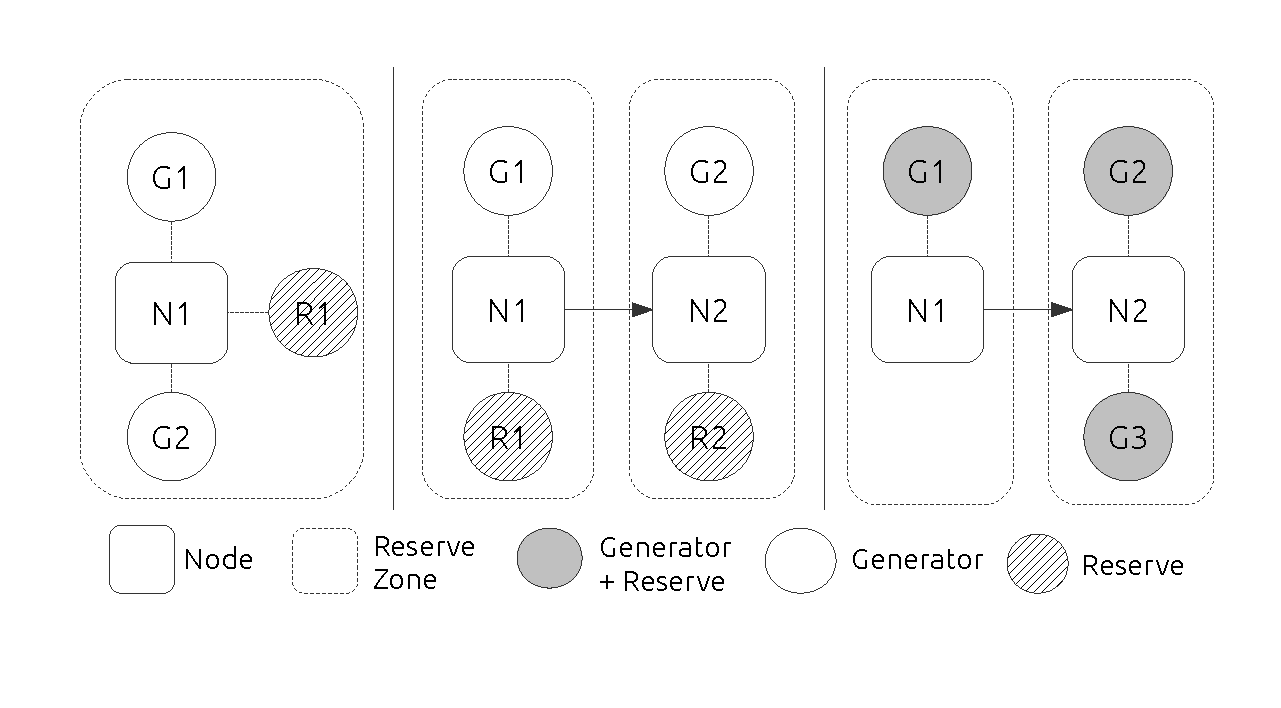
\includegraphics[width=0.95\textwidth]{img/nodal_diagram.pdf}
\caption{Some Case Studies to illustrate different mechanisms of binding
constraints occurring}
\end{figure}
\end{frame}


%%%%%%%%%%%%%%%%%%%%%%%%%%%%%%%%%%%%%%%%%%%%%%%%%%%%%%
%%%%%%%%%%%%%%%%%%%%%%%%%%%%%%%%%%%%%%%%%%%%%%%%%%%%%%
\begin{frame}{Case Study Results}
Marginal Risk Setting Generator
\begin{equation}
\pi = p_{g,marginal} - \lambda
\end{equation}
Risk Constrained Transmission Line
\begin{equation}
\pi_2 = \pi_1 - \lambda_2
\end{equation}
Bathtub Constrained Transmission
\begin{equation}
\pi_2 = \dfrac{1}{1+k_{g,2}}p_{g,2} + \dfrac{k_{g,2}}{1+k_{g,2}}(\pi_1 + p_{r,2})
\end{equation}
\end{frame}

\begin{frame}{Testing These, Marginal Generator}
\begin{figure}
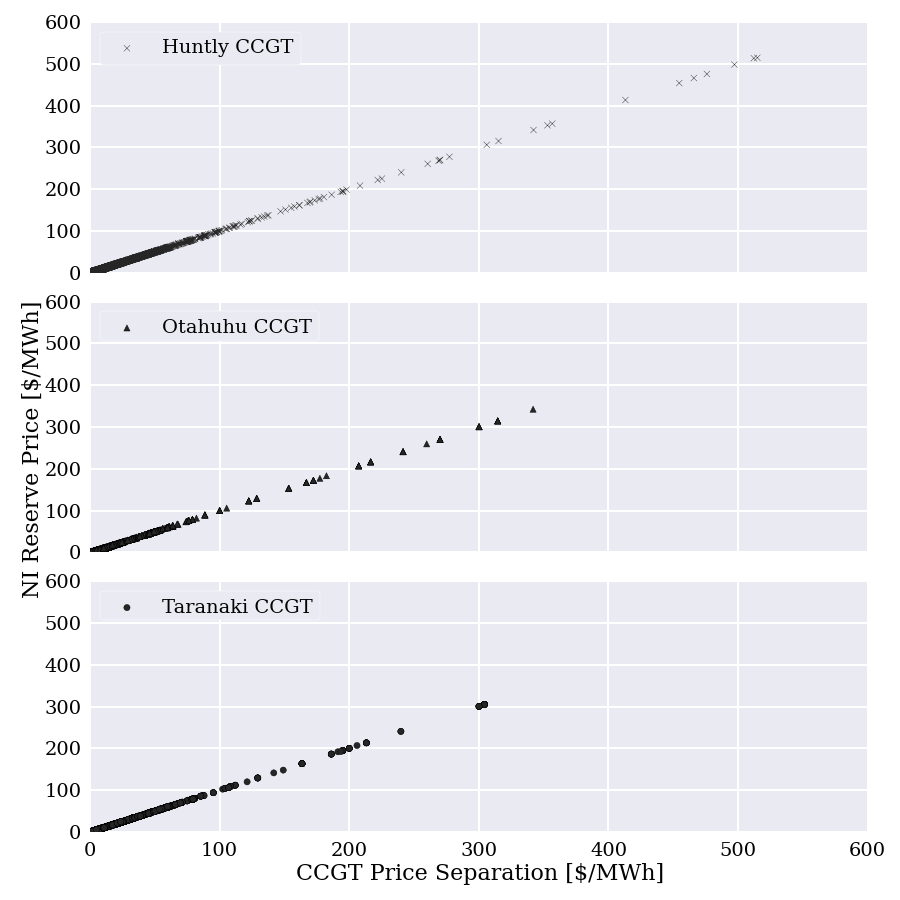
\includegraphics[scale=0.3]{img/ccgt_reserve_prices_offer_prices.png}
\caption{Reserve Constraints binding upon major CCGT Units}
\end{figure}
\end{frame}

\begin{frame}{Testing These, Marginal Transmission, NI}
\begin{figure}
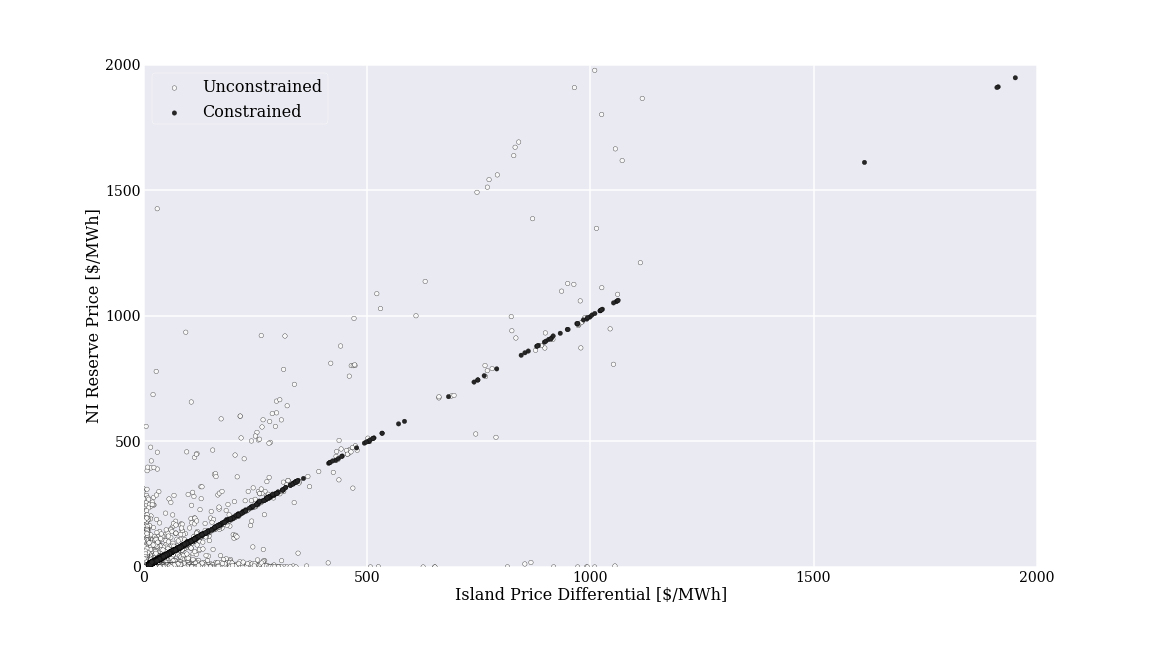
\includegraphics[width=0.95\textwidth]{img/ni_reserve_prices_island_differential.png}
\caption{Reserve Constraints Binding upon Northward HVDC Transmission}
\end{figure}
\end{frame}

\begin{frame}{Testing These, Marginal Transmission, SI}
\begin{figure}
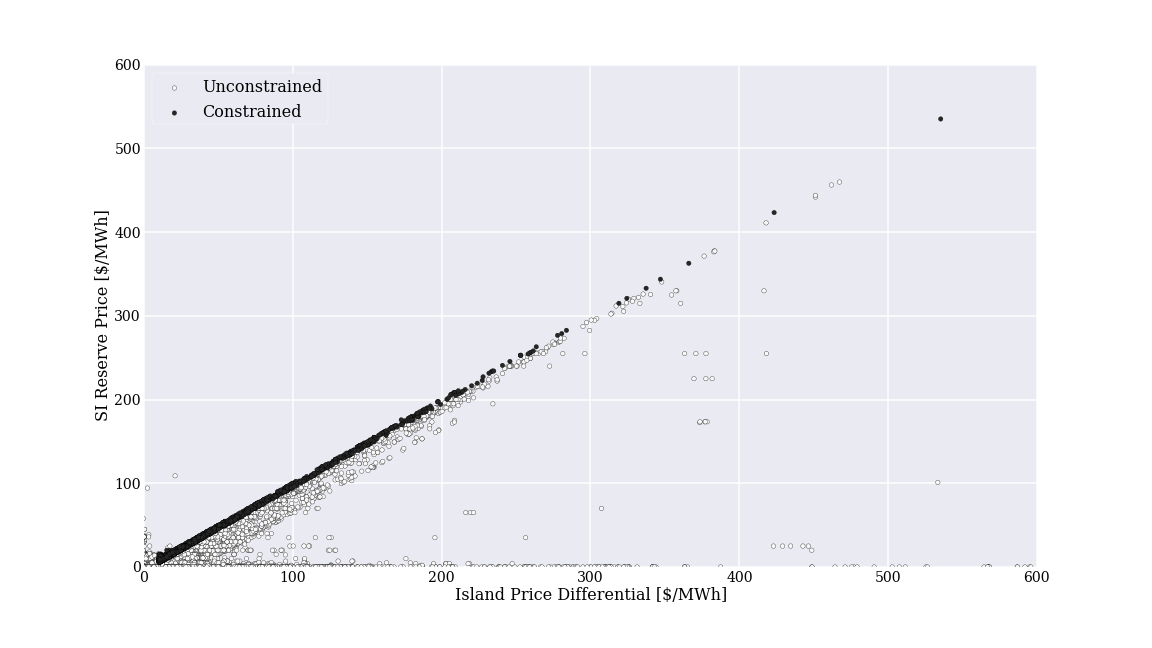
\includegraphics[width=0.95\textwidth]{img/si_reserve_prices_island_differential.png}
\caption{Reserve Constraints Binding upon Southward HVDC Transmission}
\end{figure}
\end{frame}

\begin{frame}{Testing These, Bathtub Constraints}
\begin{figure}
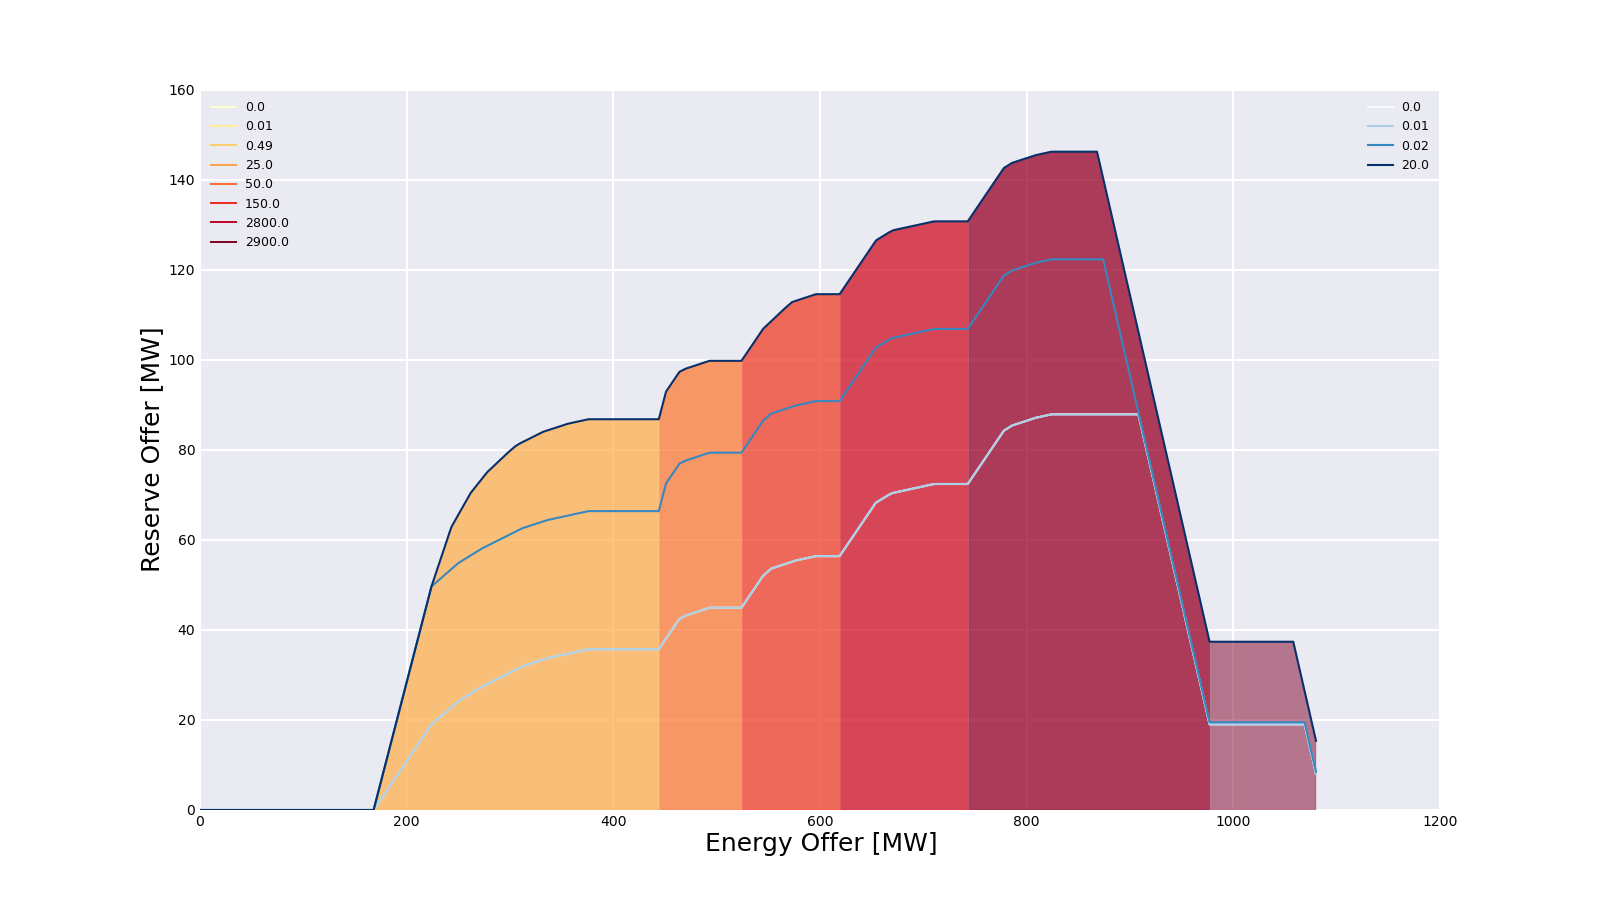
\includegraphics[width=0.95\textwidth]{img/mrpl_fan_curve.png}
\caption{Mighty River Fan Curve, TP 19, October 3 2013.}
\end{figure}
\end{frame}

\begin{frame}{Impact on the market}
\begin{figure}
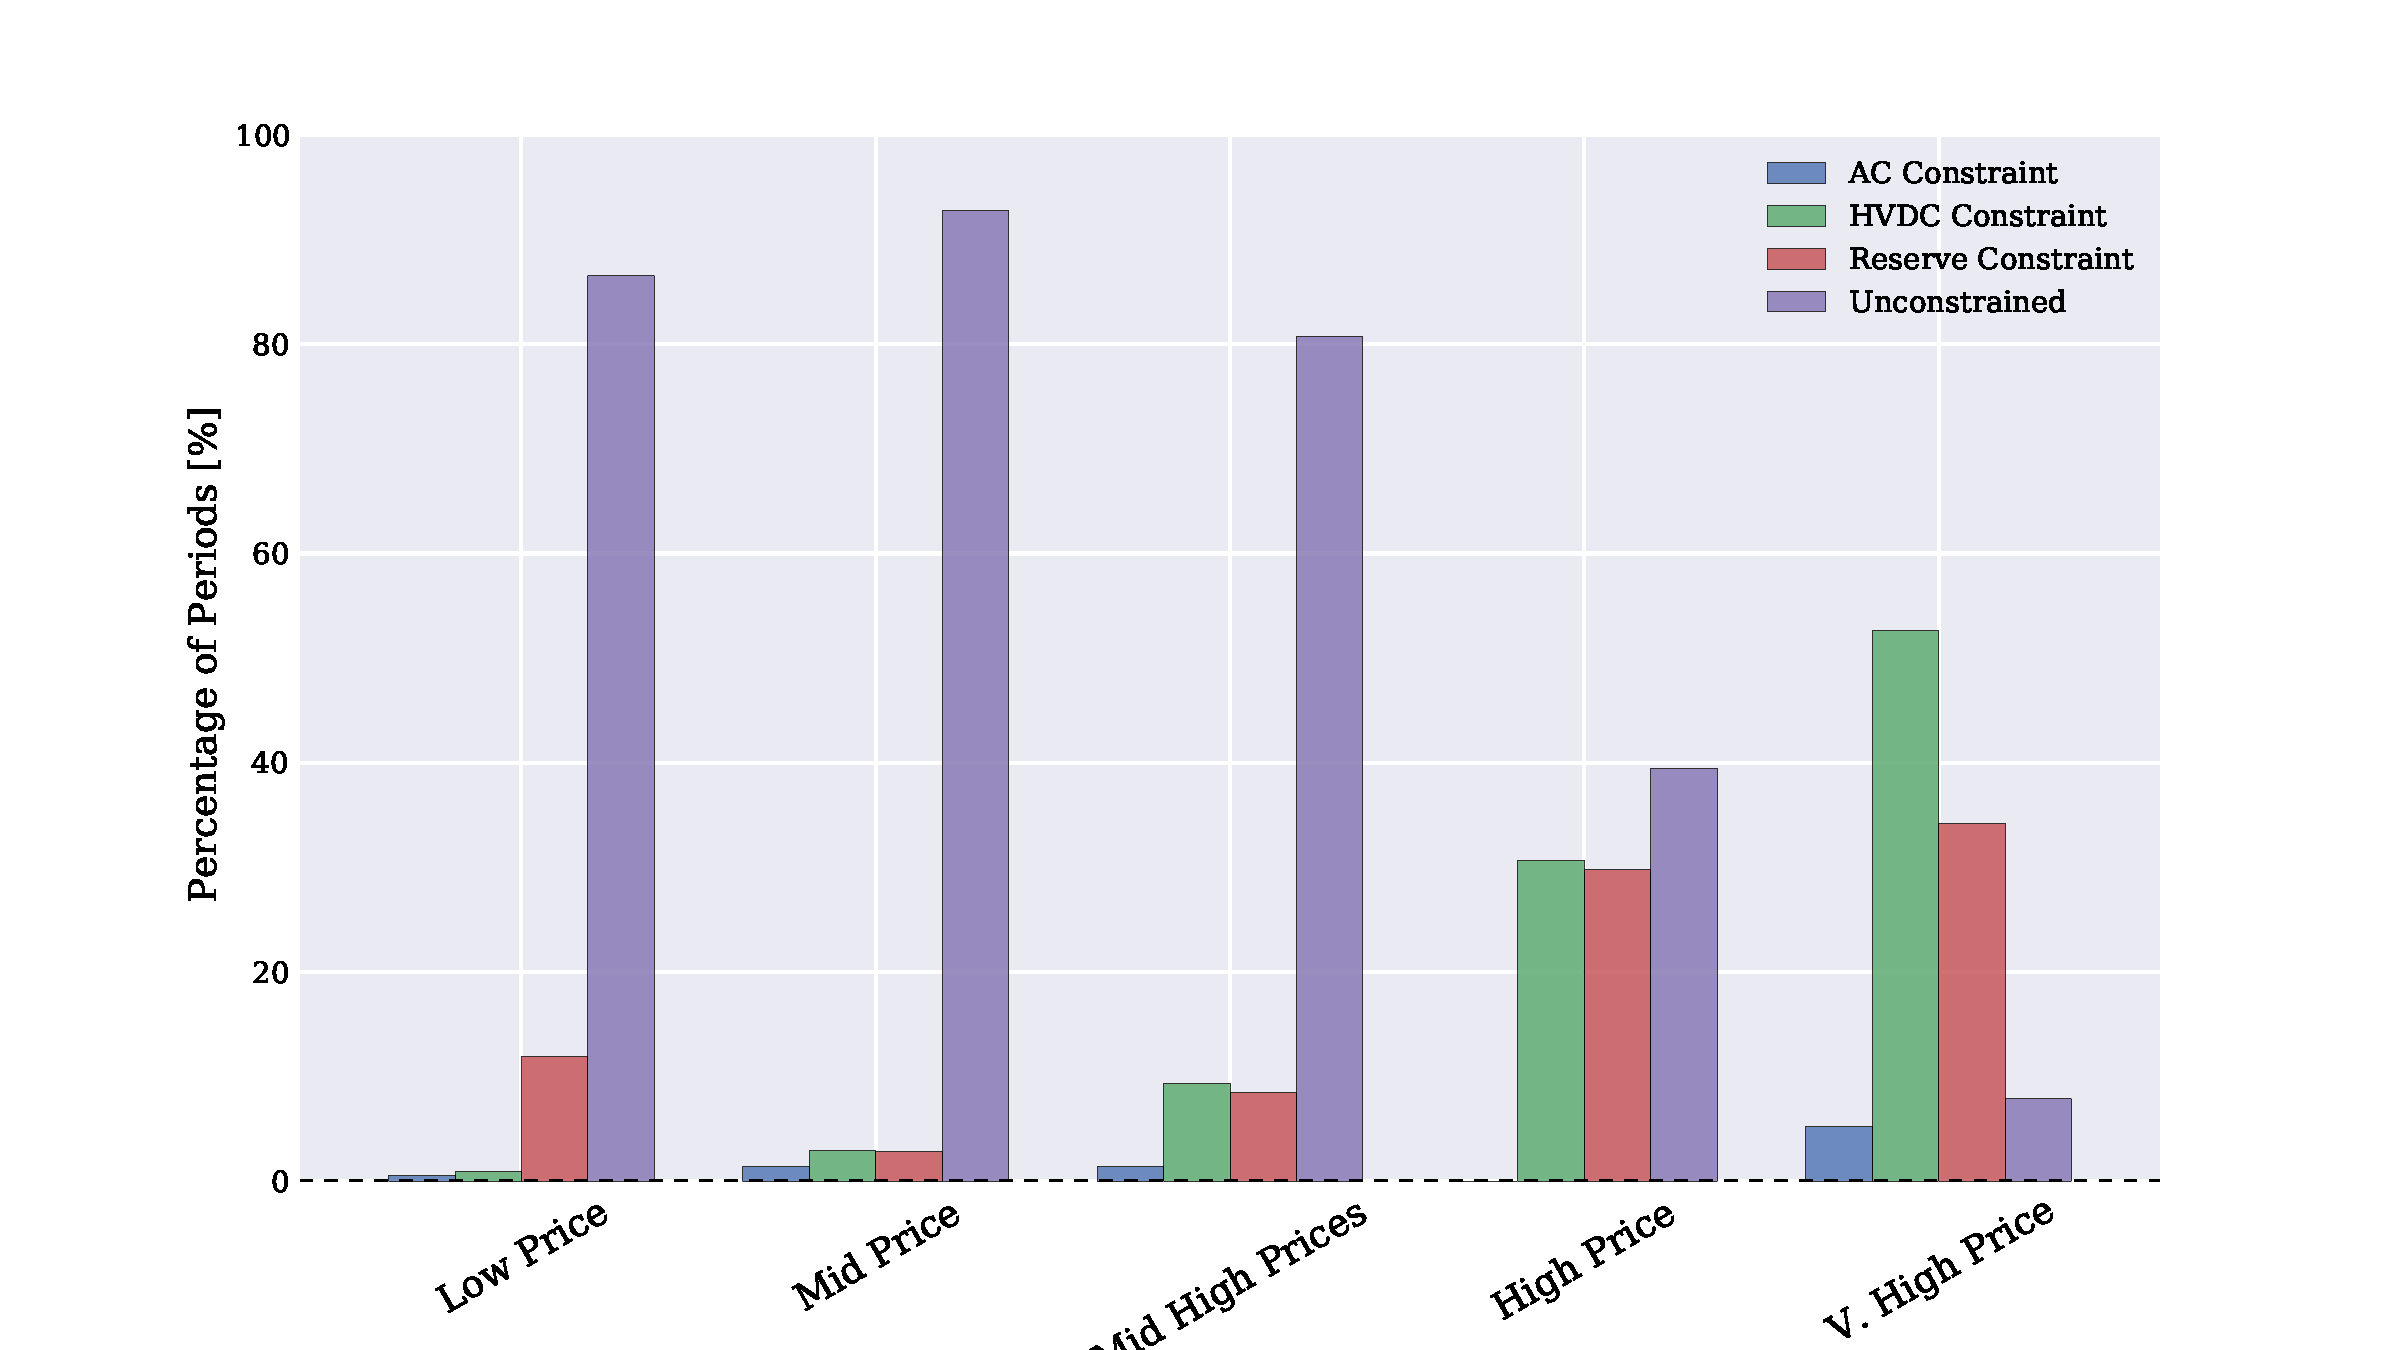
\includegraphics[width=0.95\textwidth]{img/constrained_periods_analysis.pdf}
\caption{Aggregate assessment of constraints in the New Zealand Market}
\end{figure}
\end{frame}


%%%%%%%%%%%%%%%%%%%%%%%%%%%%%%%%%%%%%%%%%%%%%%%%%%%%%%
%%%%%%%%%%%%%%%%%%%%%%%%%%%%%%%%%%%%%%%%%%%%%%%%%%%%%%
\subsection{frame 1}
\begin{frame}{frame 1}

\end{frame}

%%%%%%%%%%%%%%%%%%%%%%%%%%%%%%%%%%%%%%%%%%%%%%%%%%%%%%
%%%%%%%%%%%%%%%%%%%%%%%%%%%%%%%%%%%%%%%%%%%%%%%%%%%%%%
\section{\scshape Results}
\subsection{Frame 1}
\begin{frame}{Frame 1}

\end{frame}

\end{document}
